\documentclass{beamer}

\usepackage{default}

\usetheme{Malmoe}
\usecolortheme{dolphin}

\title{Extensions on Contract Net Protocol for AGVs}
\subtitle{Multi-Agent Systems}

\author{\textbf{Jens Claes} \and Victor Le Pochat}
\date{June 6, 2016}

\begin{document}
	\frame{\titlepage}

	\section{Introduction}
	
	\begin{frame}{Objectives \& Hypotheses}
		\begin{itemize}
		\item CNET vs CNCP vs DynCNET
		\item Hypotheses:
			\begin{itemize}
			\item Compare
				\begin{itemize}
				\item Profit
				\item Delivery time
				\item \# clients undelivered
				\item Message count
				\end{itemize}
			\item Influence on profit
				\begin{itemize}
				\item \# Drones
				\item \# Warehouses
				\item \# Clients
				\end{itemize}
			\end{itemize}
		\end{itemize}
	\end{frame}
	\note{Hypotheses zelf gewoon zeggen}
		
	\begin{frame}{Setting}
		\begin{itemize}
		\item Package delivery company
		\item Drones (UAV)
		\item Battery-constrained
		\item Warehouses
		\item 2 types clients
		\item Fines
		\end{itemize}
	\end{frame}

	\section{Theory}
	
	\begin{frame}{Contract Net Protocol (CNET)}
		\begin{itemize}
			\item Assigning tasks to (idle) agents
			\item Distributed manner
			\item Contract negotiation between initiator and participant
			\begin{itemize}
				\item I: Task announcement
				\item P: Bid on best
				\item I: Awarding
				\item P: Execution
			\end{itemize}
		\end{itemize}
	\end{frame}
	
%	\begin{frame}{Contract Net Protocol (CNET)}
%	  \begin{columns}[T] % the "c" option specifies center vertical alignment
%	  \column{.5\textwidth} % column designated by a command
%	   Negotiation protocol
%	  \column{.5\textwidth}
%	   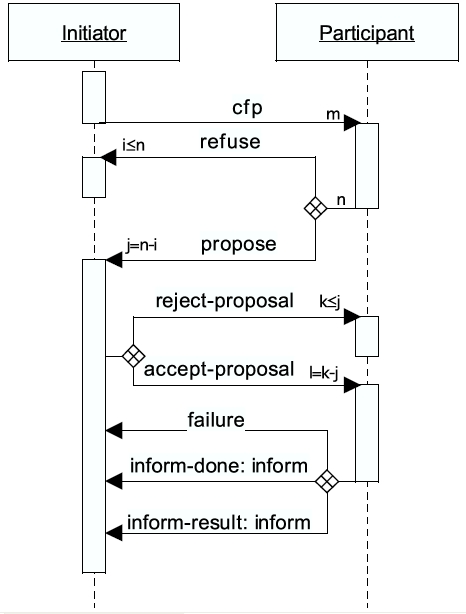
\includegraphics[width=\columnwidth]{FIPA-CNET}
%	  \end{columns}
%	\end{frame}

	\begin{frame}{Contract Net with Confirmation (CNCP)}
		\begin{itemize}
			\item Delayed commitment
			\item Bid on all
			\item Accept/Decline when awarded
		\end{itemize}
	\end{frame}

	\begin{frame}{Dynamic Contract Net (DynCNET)}
		\begin{itemize}
			\item Allow contract switching
				\begin{itemize}
				\item Initiator
				\item Participant
				\end{itemize}
			\item Preparation vs execution
			\item Oscillation
		\end{itemize}
	\end{frame}
	
	\begin{frame}{Other extensions}
		\begin{itemize}
			\item Prebidding vs Definitive bidding (Aknine et al.)
			\item Iterated Contract Net
			\item Leveled commitment
		\end{itemize}
	\end{frame}
	
	\section{Design}
%	\begin{frame}{MAS design}
%		\begin{itemize}
%			\item Clients have an order
%			\item Drone takes up order
%			\item Drone collects package at warehouse
%			\item Drone flies to client and delivers package
%		\end{itemize}
%	\end{frame}
	
	\begin{frame}{MAS design}
		\begin{itemize}
			\item Goal: maximize profit
			\item Allocate task to most suitable drone
			\item Find cheapest warehouse
			\item Minimize crashes
			\begin{itemize}
				\item Keep battery charged
				\item Poisson distribution
			\end{itemize}
			\item Deliver on time
			\item Cost estimation
				\begin{itemize}
				\item Price package
				\item Price battery charge
				\item Price failed drone
				\item Price client
				\end{itemize}
		\end{itemize}
	\end{frame}
	
	\begin{frame}{MAS design comparison}
		\begin{itemize}
			\item Simplified task announcement: only order
			\item CNET: only 1 bid
			\item Implemented RefusalReason (+ nextAvailableTime)
			\item CNCP: 1 message + reannounce task
			\item DynCNET: no prevention of oscillation
		\end{itemize}
	\end{frame}
	
	\section{Experiments}
	\begin{frame}{Experiments}
		\begin{itemize}
			\item ANOVA
			\item Games-Howell vs TukeyHSD
		\end{itemize}
	\end{frame}
	
	\section{Conclusion}
	\begin{frame}{Conclusion}
		\begin{itemize}
			\item
		\end{itemize}
	\end{frame}
	
\end{document}
